\documentclass{article}
\usepackage{graphicx,xy,amsmath,amssymb,amsthm,physics,mathtools,tcolorbox,hyperref}
\usepackage{xepersian}
\settextfont{XB Niloofar}
\title{	
	پیش گزارش ششم درس آزمایشگاه اپتیک - دکتر مهدوی
	\\
	\small
	موضوع آزمايش: پراش فرانهوفر
}
\author{
حسین محمدی 
\\
۹۶۱۰۱۰۳۵
}
\begin{document}
\maketitle
\section{هدف آزمایش}
در این آزمایش قصد داریم که پراش در رژیم فرانهوفر را بررسی کنیم و پراشنده های متفاوتی را در مسیر نور قرار می دهیم و طرح های گوناگونی را که روی پرده مشاهده می شود را می بینیم. سپس از روی مشخصاتی که این طرح ها دارند، می توانیم به برخی از ویژگی های چینش آزمایش و پراشنده پی ببریم.
\begin{enumerate}
	\item
	در آزمایش اول که پراش از تک شکاف است، عرض تک شکاف را می توان حاصل کرد.
	\item
	در آزمایش دوم پراش از پراشنده مستطیلی را مشاهده می کنیم.
	\item
	در آزمایش سوم، پراش از سیم را مشاهده می کنیم و قادر هستیم قطر سیم را محاسبه کنیم.
	\item
	در آزمایش چهارم، پراش از لبه مستقیم را می بینیم.
	\item
	آزمایش پنجم پراش از روزنه دایره ای شکل است. فاصله ی فریز ها را به دست می آوریم و نسبت بین آن ها را پیدا می کنیم.
	\item
	در آزمایش ششم و هفتم و هشتم هم پراش از روزنه مثلث شکل و روزنه 
	\lr{v}
	شکل و شبکه توری را مشاهده می کنیم.

\end{enumerate}
\section{رژیم فرانهوفر و رژیم فرنل}
بر حسب اينکه فاصله بين چشمه نور و پرده در چه حدودی باشد پديده پراش را به دو
قسمت پراش فرانهوفر و پراش فرنل تقسيم می کنند. 
\begin{itemize}
	\item
	در پراش فرانهوفر که موضوع اين آزمايش است چشمه نور
	و پرده هر دو در فاصله زيادی از سطح پراش دهنده قرار دارند، يعنی پرتوهائی که به روزنه ی پراشنده میرسند
	موازی بوده و جبهه موج تخت خواهد بود. پراش حاصل از این رژیم، حاصل تداخل امواج موازی خواهد بود. (گاهی از یک عدسی برای موازی کردن پرتوهای نور استفاده می شود که در این صورت می توان با نزدیک قرار دادن چشمه نور به روزنه، بازهم در رژیم فرانهوفر بود.)
	\item
	 در پراش فرنل چشمه
	نور و پرده ای که پراش روی آن تشکيل میشود در فاصله محدود از مانعی که سبب پراش می شود قرار
	دارند و امواجی که بوسيله مانع محدود می شوند کره هایی به مرکز منبع نورانی هستند. پس پراش حاصل از این رژیم حاصل تداخل امواج با جبهه های کروی هستند.
\end{itemize}
در شکل 
\ref{Fig1}
تفاوت این دو را می بینید.
\begin{figure}[h]
	\centering
	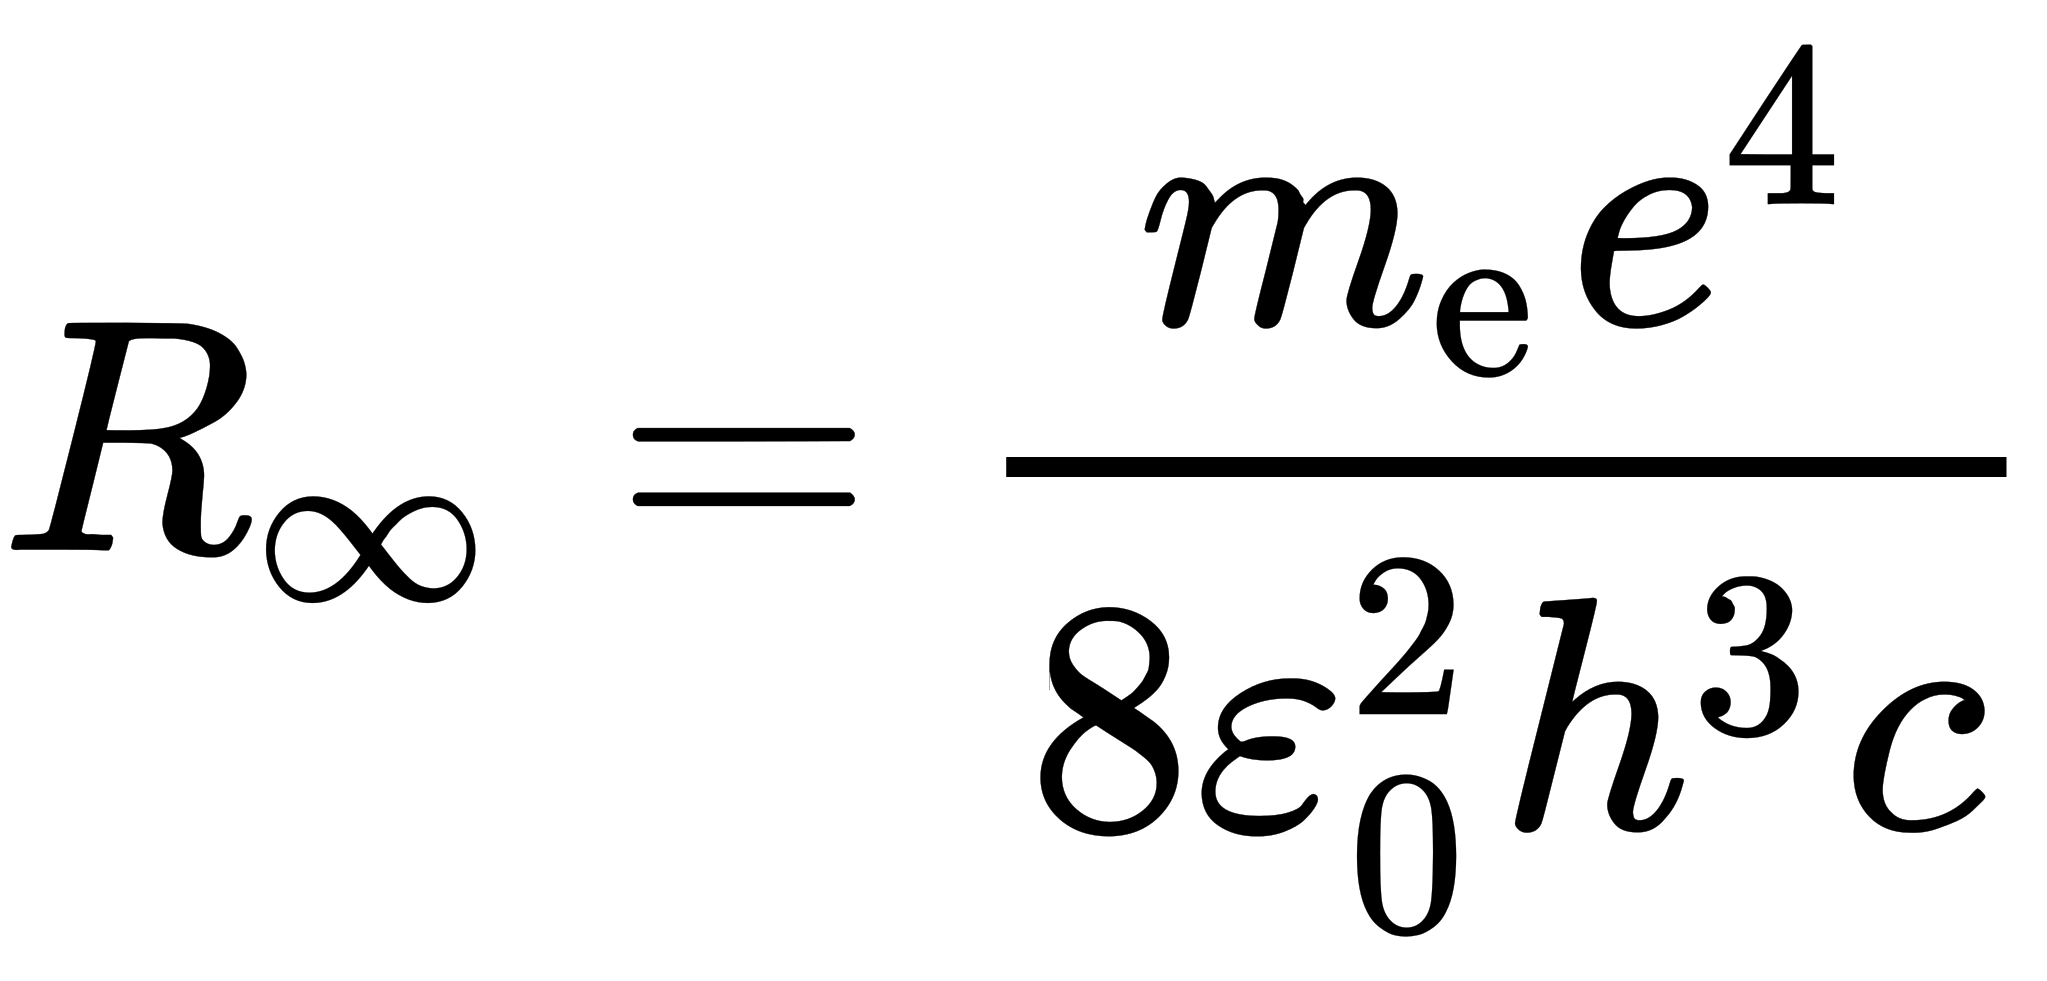
\includegraphics[scale=0.5]{1.jpg}
	\caption{پراش در رژیم فرانهوفر و فرنل}
	\label{Fig1}
\end{figure}
\section{ اثر افزایش عرض تک شکاف در طرح پراش فرانهوفر}
مطابق رابطه ی 
$d = \frac{\lambda D}{i}$
، با افزایش عرض تک شکاف یعنی 
$d$
، 
فاصله ی بین دو نوار تاریک یا روشن متوالی یعنی 
$i$
 کاهش می یابد و این نوار ها به هم نزدیک تر شده و فشرده تر می گردند.
\section{شکل ریاضی طرح پراش یک روزنه دایروی}
شکل
\ref{Fig2}
طرح پراش را نشان می دهد.
\begin{figure}[h]
	\centering
	\includegraphics[scale=0.5]{2.jpg}
	\caption{طرح پراش روزنه دایروی در رژیم فرانهوفر}
	\label{Fig2}
\end{figure}
در اینجا مقصود این است که به طور تقریبی معادلات دوایری را که در شکل 
\ref{Fig2}
می بینیم، مطرح کنیم.

\noindent
مطابق دستور کار، سه دایره اول دارای معادله زیر هستند:
\[
r_1 = 0.61 \frac{\lambda D}{d}
\]
\[
r_2 = 1.12 \frac{\lambda D}{d}
\]
\[
r_3 = 1.62 \frac{\lambda D}{d}
\]
\section{مشکلات پراش در رصد ستارگان و میکروسکوپ}
منبع اصلی اطلاعاتی که در نجوم به دست می آید تلسکوپ ها هستند؛ اما نوری که از تلسکوپ عبور می کند دچار پراش می شود، دقیقا به همان شیوه ای که در این آزمایش دیدیم، چون منبع نور در بی نهایت است و قرار است که از یک روزنه کوچک به چشم بیننده برسد، پس نور دچار پراش خواهد شد.

\noindent
این پراش، قدرت تفکیک یا رزولوشن تلسکوپ را محدود می کند؛ به تصویر 
\ref{Fig3}
توجه کنید تا بهتر متوجه این نکته بشوید.

\begin{figure}[h]
	\centering
	\includegraphics[scale=0.95]{3.jpg}
	\caption{قدرت تفکیک تک شکاف}
	\label{Fig3}
\end{figure}

در طراحی تلسکوپ ها معیاری به عنوان «معیار رایلی» هست که بر طبق آن هر چه قطر تلسکوپ را بیشتر کنیم، قدر تفکیک و بازنمایی تصویر بهتر می شود. پس مشکل «قدرت تفکیک» که در اثر پراش به وجود می آید، از مشکلات اپتیکی ساخت تلسکوپ ها است.

\noindent\\
در میکروسکوپ ها هم چنین مشکلی پیش می آید و پراش قدر تفکیک را کم می کند.
در تصویر 
\ref{Fig4}
نمونه این اثر را می بینید:
\begin{figure}[h]
	\centering
	\includegraphics[scale=0.75]{4.jpg}
	\caption{قدرت تفکیک میکروسکوپ}
	\label{Fig4}
\end{figure}
به همین خاطر برای دقیقتر شدن این میکروسکوپ ها از روش های تداخل سنجی و تحلیل سیگنال و روش های رایانه ای بهره می برند
\LTRfootnote{https://www.microscopyu.com/techniques/super-resolution/the-diffraction-barrier-in-optical-microscopy}
.




























\end{document}